%% SECTION 9: ASSUMPTION E - COMPRESSION THEORY
%% ============================================================
\section{Assumption E: Compression Theory and Minimum Functional Description Length}

\textbf{Assumption E: Removing accidental human degrees of freedom reduces effective representation entropy, legal action-space, and training-token demand.} Agent-first canonical code is not a source minifier. It is a canonical coding theory for software behavior. The raw corpus contains many strings for the same behavior because humans choose different languages, frameworks, folders, continuous-integration workflows, repository settings, dependency wrappers, migration rituals, and naming schemes. The canonical standard maps that equivalence class to a smaller canonical space, then constrains future edits through schemas, proof lanes, and semantic patch cells.

Let $X$ be raw human-code representations and $Z$ be canonical behavior representations. Let $Y$ be observable software behavior. The canonical standard is useful only if the canonical map preserves behavior while reducing irrelevant representation entropy:
\begin{equation}
  H(Z \mid Y) \ll H(X \mid Y).
\end{equation}
This is the formal version of ``one governed way per supported software class.'' For a supported concern, if two implementations expose the same behavior and invariants, they should not remain two equally privileged training targets. One interface becomes canonical; independent implementations, port traces, negative paths, compatibility fixtures, or excluded artifacts remain only when they carry evidence, diversity, governance, or security value.

\subsection{Compression Accounting Protocol}

All ranges in this paper are priors or targets until promoted by measurement. A range becomes measured only when the numerator, denominator, task distribution, model, evidence tier, and confidence interval are reported. For task distribution $\tau$ and target quality $q$:
\begin{align}
R_{\mathrm{source}}(\tau)
  &= \frac{T_{\mathrm{raw\ source}}(\tau)}
          {T_{\mathrm{canonical\ source}}(\tau)}, \\
R_{\mathrm{train}}(q,\tau)
  &= \frac{D_{\mathrm{raw}}(q,\tau)}
          {D_{\mathrm{canonical}}(q,\tau)}, \\
R_{\mathrm{reason}}(\tau)
  &= \frac{T_{\mathrm{reason+tool,raw}}(\tau)}
          {T_{\mathrm{reason+tool,canonical}}(\tau)}, \\
R_{\mathrm{change}}(\tau)
  &= \frac{C_{\mathrm{verified\ change,raw}}(\tau)}
          {C_{\mathrm{verified\ change,canonical}}(\tau)}.
\end{align}
Composite ratios cannot be multiplied unless a fitted causal model validates separability on held-out paired tasks. This is especially important for language collapse, framework collapse, generated truth, behavior cells, and proof lanes, which often remove the same tokens, edits, or reasoning loops.

The strongest effect is not literal token shrinkage. The strongest effect is action-space and reasoning-space collapse. A raw repository asks an agent to infer where code lives, what is generated, which tests matter, whether a migration is safe, how the CI system encodes permissions, what dependency path is acceptable, and what local naming convention should be preserved. A canonical repository turns those choices into explicit law. That law may add some metadata tokens, but it removes entire families of invalid edits, failed repair loops, and rediscovery reasoning.

\begin{table*}[t]
\caption{Canonical Reduction Denominators}
\label{tab:denominators}
\centering
\footnotesize
\begin{tabularx}{\textwidth}{p{0.22\textwidth}p{0.18\textwidth}X}
\toprule
Axis & Moonshot range & Meaning \\
\midrule
Literal source-token & \conrange{$2\times$--$8\times$ conservative} & Physical source shrinkage from generation, cells, and fewer duplicate surfaces. \\
Effective representation-space & $40\times$--$150\times$ central & Fewer valid encodings for the same supported behavior. \\
Agent action-space & \aggrange{$1{,}000\times$--$100{,}000\times$ high-end} & Fewer legal files, edits, workflows, proof lanes, migration paths, dependency choices, and generated-zone mistakes. \\
Reasoning-token space & $3\times$--$50\times$ hypothesis & Fewer planning, tool, architecture-discovery, retry, and repair tokens per accepted change. \\
Retry/review loop & $3\times$--$50\times$ hypothesis & Fewer failed tests, invalid edits, ambiguous reviews, rollback surprises, and proof reruns. \\
Training-token budget & $30\times$--$150\times$ hypothesis & Fewer examples needed to reach target canonical accuracy, conditional on paired scaling curves. \\
Cost per verified correct change & $3\times$--$100\times$ hypothesis & End-to-end cost after foundry, verification, serving, reasoning, failed-loop, and maintenance amortization. \\
\bottomrule
\end{tabularx}
\end{table*}

\begin{figure*}[t]
\centering
\scriptsize
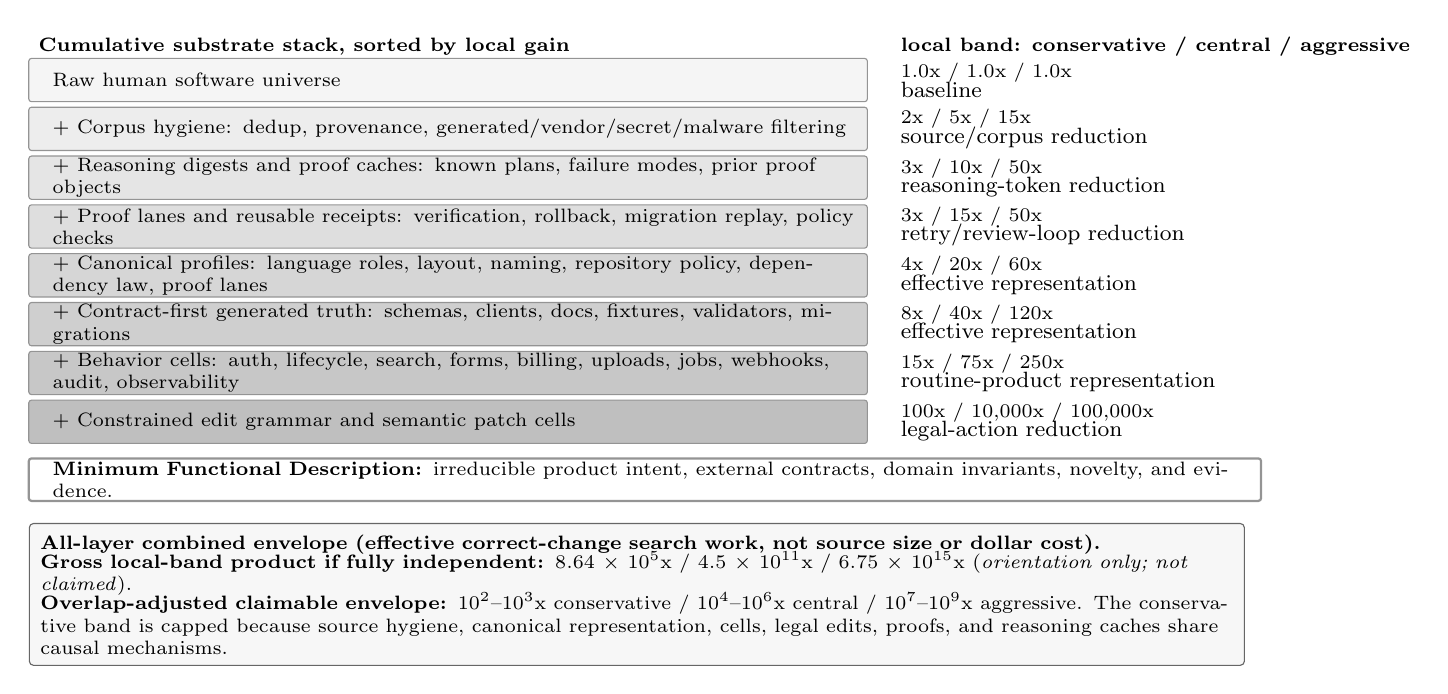
\begin{tikzpicture}[
  x=1cm,
  y=1cm,
  every node/.style={font=\scriptsize},
  layer/.style={draw=black!42, rounded corners=1pt},
  summary/.style={draw, rounded corners=1.5pt, align=left, inner sep=4pt}
]
\def\stacklayer#1#2#3#4#5#6#7{%
  \draw[layer,fill=#7] (0,#1) rectangle (10.65,#1+0.55);
  \node[anchor=west,align=left,text width=10.2cm] at (0.18,#1+0.275) {#2};
  \node[anchor=west,align=left,text width=4.7cm] at (10.95,#1+0.275) {\conrange{#3} / #4 / \aggrange{#5}\\[-1pt]{\footnotesize #6}};
}
\node[anchor=west,font=\scriptsize\bfseries] at (0,7.05) {Cumulative substrate stack, sorted by local gain};
\node[anchor=west,font=\scriptsize\bfseries] at (10.95,7.05) {local band: \conrange{conservative} / central / \aggrange{aggressive}};
\stacklayer{6.35}{Raw human software universe}{1.0x}{1.0x}{1.0x}{baseline}{black!4}
\stacklayer{5.73}{+ Corpus hygiene: dedup, provenance, generated/vendor/secret/malware filtering}{2x}{5x}{15x}{source/corpus reduction}{black!7}
\stacklayer{5.11}{+ Reasoning digests and proof caches: known plans, failure modes, prior proof objects}{3x}{10x}{50x}{reasoning-token reduction}{black!10}
\stacklayer{4.49}{+ Proof lanes and reusable receipts: verification, rollback, migration replay, policy checks}{3x}{15x}{50x}{retry/review-loop reduction}{black!13}
\stacklayer{3.87}{+ Canonical profiles: language roles, layout, naming, repository policy, dependency law, proof lanes}{4x}{20x}{60x}{effective representation}{black!16}
\stacklayer{3.25}{+ Contract-first generated truth: schemas, clients, docs, fixtures, validators, migrations}{8x}{40x}{120x}{effective representation}{black!19}
\stacklayer{2.63}{+ Behavior cells: auth, lifecycle, search, forms, billing, uploads, jobs, webhooks, audit, observability}{15x}{75x}{250x}{routine-product representation}{black!22}
\stacklayer{2.01}{+ Constrained edit grammar and semantic patch cells}{100x}{10,000x}{100,000x}{legal-action reduction}{black!25}
\draw[layer,fill=white,thick] (0,1.28) rectangle (15.65,1.82);
\node[anchor=west,align=left,text width=15.25cm] at (0.18,1.55) {\textbf{Minimum Functional Description:} irreducible product intent, external contracts, domain invariants, novelty, and evidence.};

\node[summary,fill=black!3,draw=black!60,text width=15.15cm,anchor=north west] at (0,1.00) {
\textbf{All-layer combined envelope (effective correct-change search work, not source size or dollar cost).}\\[-1pt]
\textbf{Gross local-band product if fully independent:}
\conrange{$8.64\times10^{5}\mathrm{x}$} / $4.5\times10^{11}\mathrm{x}$ / \aggrange{$6.75\times10^{15}\mathrm{x}$}
(\textit{orientation only; not claimed}).\\[-1pt]
\textbf{Overlap-adjusted claimable envelope:}
\conrange{$10^{2}$--$10^{3}\mathrm{x}$ conservative} /
$10^{4}$--$10^{6}\mathrm{x}$ central /
\aggrange{$10^{7}$--$10^{9}\mathrm{x}$ aggressive}. The conservative band is capped because source hygiene,
canonical representation, cells, legal edits, proofs, and reasoning caches share causal mechanisms.
};
\end{tikzpicture}
\caption{Canonical Compression Cascade: From Human-Code Entropy to Minimum Functional Description. The stack starts at the 1.0$\times$ raw baseline and then adds layers sorted by conservative local gain, with ties ordered by central gain. The right column gives the local hypothesis band for each layer. The final block combines all row multipliers two ways: a gross independent-axis product for orientation, and a deliberately smaller overlap-adjusted envelope for effective correct-change search work. The local ranges are measured on different denominators and are not naively multiplied. Training time, inference cost, and verified-change cost remain separate outcome denominators.}
\label{fig:compressioncascade}
\end{figure*}

The final block in Figure~\ref{fig:compressioncascade} deliberately separates the raw independence bound from the claimable combined range. The conservative envelope is not the product of every row. It is anchored by constrained legal edits plus a small number of independent reductions in representation, retry, and reasoning work; stronger bands require evidence that those reductions remain separable on paired tasks.

Contract-first generation is the first large step toward that limit: OpenAPI and Protocol Buffers are existing examples of schema-owned surfaces that generate clients, validators, and transport bindings instead of hand-maintaining parallel representations~\cite{openapi31,protobufOverview}. Semantic patch systems such as Coccinelle and constrained generation systems such as XGrammar show complementary directions: patches and outputs can be represented as structured grammars rather than unconstrained text~\cite{coccinelle,xgrammar}.

The theoretical limit is \textbf{Minimum Functional Description Length}: a frontier over canonical specifications, evidence bundles, and renderers, not a magical globally shortest program. For substrate $\mathcal{S}$, preservation threshold $\tau$, behavior target $y$, proof/evidence bundle $\Pi$, renderer $\mathcal{R}_{\mathcal{S}}$, and observable-behavior oracle $\mathcal{O}$:
\begin{multline}
\operatorname{MFDL}_{\mathcal{S},\tau}(y)=
\min_{z\in\mathcal{Z}_{\mathcal{S}}}
\left(|z|+\lambda|\Pi(z)|+\mu|\mathcal{R}_{\mathcal{S}}|\right)\\
\text{s.t.}\quad
\mathcal{O}(\mathcal{R}_{\mathcal{S}}(z),y)\ge\tau.
\end{multline}
This is not code golf and not syntax preference. It is the end state where bespoke code appears only when the behavior is novel. Routine product behavior becomes behavior graph operations, cell composition, generated surfaces, policies, schemas, migrations, semantic patches, and proof receipts. In that limit, the model is no longer trained to imitate the long tail of human implementation choices. It is trained to operate a constrained software machine.

\textbf{Falsification:} Assumption E fails if paired raw/canonical corpora do not reduce measured source tokens, identifier entropy, AST-pattern entropy, path grammar, proof-loop count, perplexity, or action branching on target software classes.

%% ============================================================
